\PassOptionsToPackage{dvipdfmx}{graphicx}% NOTE: only for Japanese
\PassOptionsToPackage{dvipdfmx}{xcolor}% NOTE: only for Japanese
\documentclass[sip,biber]{now-journal}
\addbibresource{IEEEabrv.bib}
\addbibresource{ref.bib}

\usepackage[nolist,nohyperlinks]{acronym}
\usepackage{amsfonts}
\usepackage{bm}
\usepackage{mathtools}
\usepackage{siunitx}
\usepackage[skip=1pt]{subcaption}

% reload hyperref
\usepackage[colorlinks=true, allcolors=blue, plainpages=false, pdfpagelabels=true]{hyperref}
\usepackage{breakurl}

% cleveref setting
\usepackage[capitalise]{cleveref}
\crefformat{equation}{(#2#1#3)}
\Crefformat{equation}{#2Equation~(#1)#3}
\crefformat{section}{Section~#2#1{}#3}
\crefname{algorithm}{Algorithm}{Algorithms}
\crefname{equation}{}{}
\crefname{figure}{Figure}{Figures}
\crefname{section}{Section}{Sections}
\def\crefrangeconjunction{--}

% psuedo codes
\usepackage{xcolor}
\usepackage[theorems,skins]{tcolorbox}
\usepackage{tabularx}
\usepackage{pseudo}
\newtcbtheorem[crefname = {Algorithm}{algorithms}]{algorithm}{Algorithm}{pseudo/booktabs, float=t, theorem hanging indent=0pt}{alg}
\pseudodefinestyle{fullwidth}{
    begin-tabular=
    \tabularx{\textwidth}[t]{@{}
        r                                          % Labels
        >{\leavevmode\pseudosetup}                 % Indent, font, ...
        X                                          % Code (flexible)
        >{\leavevmode} % Comment styling
        p{0.20\textwidth}                           % Comments (fixed)
        @{}},
    end-tabular=\endtabularx,
}
\pseudoset{%
   fullwidth,
   kwfont=\sffamily\bfseries,
   font=\kwfont,
   prfont=\textsf,
   hsep=.3em,
   indent-mark,
   indent-mark-shift=.5em,
   indent-length=1em,
   line-height=1.5,
   ct-left=\hfill\texttt{//}~,
   ct-right=,
   % label=\textcircled{\ttfamily\scriptsize\arabic*},
   label=,
   % ref,
}

% Align euqality or replacement in pseudo codes
% ref: https://latex.org/forum/viewtopic.php?t=26363
\usepackage{xparse}
\DeclareDocumentCommand{\psm}{m O{$\gets$}}{% pseudocode-math
  {\hphantom{$W_{k,f,t - 1}$}\llap{#1}~#2}%
  % {\rlap{#1}\hphantom{$W_{k,f,t}$}#2}%
}

% Original style files
\usepackage{bsssym}
\newcommand{\todo}[1]{\textcolor{red}{#1}}

% Document information
\title{Self-Rotation-Robust Online Independent Vector Analysis with\\Sound Field Interpolation on Circular Microphone Array}
\fancyhead[LO]{\footnotesize\textit{Self-rotation-robust online independent vector analysis with sound field interpolation on circular microphone array}}
\author{Nakashima, Taishi}
\affil{Tokyo Metropolitan University, Tokyo, Japan}
\author{Wakabayashi, Yukoh}
\affil{Toyohashi University of Technology, Aichi, Japan}
\author[1]{Ono, Nobutaka}
\creditline{%
  Corresponding author: Taishi Nakashima, \href{mailto:taishi@ieee.org}{taishi@ieee.org}.
  This work was supported by JSPS KAKENHI Grant Number 21J22039 and JST CREST Grant Number JPMJCR19A3.
}

\articledatabox{
  Received XX June 2023; Revised YY Sep 2023
  ISSN XXXX-YYYY; DOI xx.yyyy/zzz.wwwwwwww\\
  \copyright 2023 T. Nakashima, Y. Wakabayashi, and N. Ono
}

\keywords{
  Blind source separation,
  online independent vector analysis,
  circular microphone array,
  sound field interpolation
}

\begin{document}

\begin{abstract}
  % 本論文では,マイクロホンアレイの回転に頑健なオンラインブラインド音源分離手法を提案する.
  % Online auxiliary-function-based independent vector analysis (OIVA)はリアルタイムBSSを実現するための有望な手法のひとつである.
  % リアルタイムBSSを実用化するためには,音源やマイクの移動といった環境の変化に対する頑健性が重要な課題である.
  % 一般的にリアルタイム処理の最中に環境の変化が起こった場合はパラメータの再推定が必要である.
  % OIVAでは音源のなめらかな移動に対して頑健かつ高い分離性能を獲得できることが示されていた.
  % しかし,OIVAはマイクの突発的な移動に対しては十分な性能が得られない.
  % そこで本論文では,円状等間隔マイクロホンアレイ(CMA)のための音場補間処理を利用したOIVAを提案する.
  % 音場補間はCMAの回転を打ち消し,パラメータの再推定を必要とせずにBSSを可能にする.
  % シミュレーション実験の結果は音場補間によりマイクが回転する状況における音源分離の頑健性が向上したことを確認した.
  In this paper, we propose a robust online blind source separation (BSS) method against the self-rotation of microphone arrays.
  Online auxiliary-function-based independent vector analysis (OIVA) is one of the promising methods for real-time BSS.
  One major issue for real-time BSS is robustness against environmental changes such as the movement of the source or microphone.
  Parameter re-estimation is generally necessary if environmental changes occur during real-time processing.
  OIVA is robust against smooth movement of sources and achieves high separation performance.
  However, OIVA does not perform well against sudden movements of microphones.
  Therefore, we employ sound field interpolation (SFI) for circular microphone arrays (CMAs) with OIVA in this paper.
  SFI cancels out the rotation of the CMA, enabling us to apply BSS without parameter re-estimation.
  Simulation experiments confirmed that SFI improves the robustness of the OIVA in situations where the microphone is rotating.
\end{abstract}

\section{Introduction}\label{sec:intro}
% ブラインド音源分離は混合信号から目的の信号を分離する技術である.
% BSSの手法はIVAやその拡張などが有名である.
% これらの手法はすべて時不変な系を仮定している.
% それに対して,実応用のためにはマイクロホンや音源の移動など系の時間変化を考慮する必要がある.
% 系の時間変化を考慮するためには,信号を短いブロックに分割し,各ブロックに対してIVAを適用するやり方が考えられる.
% ブロックバッチの手法やオンラインの手法が考えられる.
%
% オンライン独立ベクトル分析は実時間で動作し,高い性能を示した.
% オンラインAuxIVA は補聴器への応用,残響除去との組み合わせ,高速なステアリングベクトル更新など最近活発に研究されている.
% オンラインAuxIVA ではフレームごとに分離行列を推定し,音響伝達系のゆるやかな時間変化に対応できる.
% しかし,新たな音源の出現やマイクの移動など,音響伝達系の突発的な変化が起こった場合には推定が難しくなり性能が著しく低下する.
%
% 音響伝達系の突発的な変化に対応するための音響信号処理手法がいくつか提案されている.
% 円状等間隔マイクロホンアレイ(circular microphone array; CMA)の回転を考え,音場の補間により対応する手法が提案されている.
% この手法はCMAの対称性を利用することで,CMAが回転する前の音場を簡単な線形演算により推定する.
% また,ビームフォーミング \cite{Wakabayashi:2021:ICASSP} やステアリングベクトル推定 \cite{Wakabayashi:2021:ASJ:A} への応用や,
% CMAの回転角度を自己推定する手法 \cite{Lian:2021:APSIPA} も提案されている.
% そこで,本稿では,CMAが回転する状況下のブラインド音源分離に取り組む.
% 音場補間によりCMAの回転の影響を打ち消しながらオンラインでブラインド音源分離処理を行う.
Blind source separation (BSS) \cite{Makino:2018:ASS} is a technique to extract the source signals from their observed mixture.
Popular approaches for BSS include independent vector analysis (IVA) \cite{Kim:2006:ASLP,Hiroe:2006:ICA} and extensions \cite{Kitamura:2016:ASLP,Nugraha:2020:SPL,Brendel:2020:SP}.
These methods assume a time-invariant acoustic transfer system (ATS).
On the other hand, for practical applications, it is necessary to consider time variations of the ATS, such as movements of the microphone or source.
Many methods have been proposed based on block batch \cite{Koldovsky:2019:ICASSP,Koldovsky:2021:SP,Jansky:2022:ASMP} or online processing \cite{Kim:2010:CASI,Taniguchi:2014:HSCMA}.

Online AuxIVA shows high separation performance in real-time situations \cite{Taniguchi:2014:HSCMA}.
It also has been actively researched recently for applications in hearing aids \cite{Sunohara:2017:ICASSP}, joint optimization with dereverberation \cite{Ueda:2021:ICASSP}, and computationally efficient optimization \cite{Nakashima:2023:ICASSP}.
Online AuxIVA estimates demixing matrices frame-by-frame manner and can track smooth environmental changes in ATS, such as slow movement of sources.
However, sudden changes in ATS, such as the emergence of new sources or microphone movement, makes online BSS difficult and thus degrade separation performance.

\todo{AR, VR関連のサーベイ追加}

Several methods have been proposed to cope with such sudden changes in ATS.
Sound field interpolation (SFI) for circular microphone array (CMA) has been proposed to address the rotation of a CMA \cite{Wakabayashi:2023:ASLP}.
This method exploits the symmetry of the CMA to estimate the sound field before the rotation of the CMA by a simple linear operation.
Applications to beamforming \cite{Wakabayashi:2021:ICASSP} and steering vector estimation \cite{Wakabayashi:2021:ASJ:A} have also been proposed,
as well as a method for self-estimating the rotation angle of a CMA \cite{Lian:2021:APSIPA}.

In this paper, we address blind source separation in situations where a CMA rotates.
SFT cancels out the effect of the rotation, and BSS is applied in the latter stage.
As described in \cref{sec:proposed}, simply applying SFI to online BSS is computationally expensive since SFI is required for the observed signal every time frame.
In contrast, this study introduces a more straightforward method than that and demonstrates its effectiveness through experiments.
Experiments show that our proposed scheme is significantly better than the conventional online AuxIVA for the source separation task.

The rest of this paper is organized as follows.
We formulate our motivation in \cref{sec:problem}.
\Cref{sec:conventional} describes SFI and how to apply it to online BSS.
In \cref{sec:proposed}, we propose an efficient online BSS that utilizes the information before and after the rotation of CMA.
We conduct some experiments to show the efficacy of the SFI for online BSS in \cref{sec:experiment}.
Finally, \cref{sec:conclusion} concludes this paper.

\section{Problem Formulation}\label{sec:problem}
% TODO: マイクが回転する状況での音源分離の図
Let $\Src$ and $\Mic$ be the number of sources and microphones, respectively.
Also, we set the \emph{reference microphone} $\refmic = 1$ without loss of generality.
We assume that the observed signal $\Obs _{\ft}$ is modeled as
\begin{equation}
  \Obs _{\ft} = \steer _{1,\ft} \sig _{1,\ft} + \dots + \steer _{\Src,\ft} \sig _{\Src,\ft} = \sum _{\src=1} ^{\Src} \steer _{\src,\ft} \sig _{\src,\ft},\label{eq:mix}
\end{equation}
in the short-time Fourier transform (STFT) domain,
where $\freq = 1, \dots, \Freq$ denotes the frequency bin index,
$\tframe = 1, \dots, \Tframe$ denotes the time frame index,
$\sig _{\src,\ft} \in \C\; (\src = 1, \dots, \Src)$ denotes the $\src$th source signal, and
\begin{equation*}
  \steer _{\src,\ft} \coloneqq \begin{bmatrix} 1 & \str _{2\src,\ft} & \dots & \str _{\Mic\src,\ft} \end{bmatrix} ^{\top} \in \C ^{\Mic}\; (\src = 1, \dots, \Src)
\end{equation*}
denotes the steering vector of the $\src$th source signal to each microphone.
In other words, $\str _{\mic\src,\ft} \; (\mic = 2, \dots, \Mic,\; \forall \src = 1, \dots, \Src)$ corresponds to the relative transfer function from the $\src$th source to the $\mic$th microphone.
Our goal is to estimate \emph{source images} at the reference microphone $\sig _{1,\ft},\, \dots,\, \sig _{\Src,\ft}$.

Next, we assume that the observed signal $\Obs _{\ft}$ is recorded with a circular microphone array (CMA), and CMA may be rotated at angle $\rotSpat _{\tframe}$ during processing.
We consider an online BSS problem under such a situation.
We henceforth assume that the number of microphones of CMA is equal to that of sources; $\Mic = \Src$.
\renewcommand{\Mic}{\Src}%
Online blind source separation estimates demixing matrices and estimated signals using only the current and past observed signals $\Obs _{\freq,1},\, \dots,\, \Obs _{\freq,\tframe}$:
\begin{align}
  \Demix _{\ft} &= \begin{bmatrix} \demix _{1\ft} & \dots & \demix _{\Src,\ft} \end{bmatrix} ^{\hermite} \in \C ^{\Src \times \Mic}, \\
  \Est _{\ft} &= \Demix _{\ft} \Obs _{\ft} \in \C ^{\Src},
\end{align}
where $\Demix _{\ft}$ is the demixing matrix, and $\Est _{\ft}$ is the estimated signal.
Note that $\rotSpat _{\tframe}$ is assumed to be known or estimated in this paper.

Unless specified, indices $\freq,\, \tframe,$ and $\src$ always ranges from 1 to $\Freq, \Tframe,$ and $\Src$, respectively.
We omit the bounds of sets over these indices when they span the ranges.
${\{\Obs _{\ft}\}}_{\ft}$ denotes the set of $\Obs _{\ft}$ for all $\freq$ and $\tframe$, for example.
\Cref{tab:notations} summarises the notations used in this paper.
\begin{table}[t]
  \centering
  \caption{Notations}\label{tab:notations}
  \begin{tabular}{lll}
    \toprule
      Symbol & Domain & Description \\
    \midrule
      % $\Mic$               & $\Z$                     & Number of microphones \\
      $\Src$                               & $\Z$                     & Number of sources \\
      $\steer _{\src,\ft}$                 & $\C ^{\Mic}$             & Steering vector \\
      $\sig _{\src,\ft}$                   & $\C$                     & Source signal \\
      $\Obs _{\ft}$                        & $\C^{\Mic}$              & Observed signal \\
      $\Demix _{\ft}$                      & $\C^{\Src \times \Mic}$  & Demixing matrix \\
      $\Est _{\ft}$                        & $\C^{\Mic}$              & Estimated signal \\
      $\cov _{\src,\ft}$                   & $\C^{\Mic \times \Mic}$  & Covariance matrix \\
      $\forget$                            & $\{\forget \in \R \mid 0 \leq \forget < 1\}$   & Forgetting factor \\
      $\rotSpat _{\tframe}$                & $\R$                     & Spatial rotation angle \\
      $\rotSmpl$                           & $\R$                     & Rotation angle coefficient on CMA \\
      $\rotFra$                            & $\R$                     & Rotation time \\
      $\rotMat (\rotSpat _{\tframe})$      & $\R ^{\Mic \times \Mic}$ & Rotation matrix \\
      $\refpos{\Obs} _{\ft}$ & $\C^{\Mic}$ & Observes signal at \textcolor{red}{\textbf{reference position}} \\
    \bottomrule
  \end{tabular}
\end{table}

\section{Conventional Methods}\label{sec:conventional}

\subsection{Online Auxiliary-Function-Based Independent Vector Analysis}

Online AuxIVA \cite{Taniguchi:2014:HSCMA} is an online extension of AuxIVA \cite{Ono:2011:WASPAA} and estimates demixing matrices $\{\Demix _{\ft}\} _{\freq}$ at time frame $\tframe$ by minimizing the following objective function:
\begin{align}
  J _{\tframe}(\Demix _{\ft}) &= \sum _{\src = 1} ^{\Src} \demix _{\src,\ft} ^{\hermite} \cov _{\src,\ft} \demix _{\src,\ft} ^{\nohermite} - \logdet{\Demix _{\ft}} ^2, \label{eq:obj} \\
  \cov _{\src,\ft} &= \forget \cov _{\src,\ft[-1]} + (1 - \forget) \weight(\var _{\src,\tframe}) \Obs _{\ft} ^{\nohermite} \Obs _{\ft} ^{\hermite}, \label{eq:cov} \\
  \var _{\src,\tframe} &= \sqrt{\sum _{\freq=1} ^{\Freq} \lvert \demix ^{\hermite} _{\src,\ft} \Obs ^{\nohermite}_{\ft} \rvert ^2},
\end{align}
where $\weight\colon \R _{>0} \to \R _{>0}$ is defined as $\weight(\var) = \cont ' (\var) / 2 \var$ ($\cont '(\var)$ denotes the first derivative of $\cont (\var)$ with respect to $\var$),
$\cont(\var)$ is called a contrast function and derived from the probability density function of source signals,
and $\forget\; (0 \leq \forget < 1)$ is called a forgetting factor.
In this paper, we assume that $\weight (\var) = \Freq/{\var ^2}$, which represents the time-varying Gaussian distribution \cite{Ono:2012:APSIPA}.
Using the recursive update for covariance matrix \eqref{eq:cov}, we can apply efficient update methods proposed for batch AuxIVA algorithms, such as \emph{iterative projection (IP)} \cite{Ono:2011:WASPAA}, to minimize the objective function \eqref{eq:obj}.
IP cyclically updates each \emph{demixing vector} $\demix _{\src,\ft} ^{\hermite}\; (\src = 1, \dots, \Src)$ (row of the demixing matrix $\Demix _{\ft}$) using the following update rule:
\begin{align}
  \demix _{\src,\ft} &\gets (\Demix _{\ft} \cov _{\src\ft}) ^{-1} \eye _{\src} \label{eq:ip:proj}, \\
  \demix _{\src,\ft} &\gets \frac{{\demix _{\src,\ft}}}{{\sqrt{\demix _{\src,\ft} ^{\hermite} \cov _{\src,\ft} \demix _{\src,\ft}}}} \label{eq:ip:norm},
\end{align}
where $\eye _{\src} \in \R ^{\Src}$ is the canonical basis vector with the $\src$th element unity.
\Cref{alg:naive} summarises the Online AuxIVA algorithm.

\subsection{Sound Field Interpolation on Circular Microphone Array}
% TODO: 音場補間のイメージ図
This subsection briefly reviews the sound field interpolation method on circular microphone array (CMA).
We consider a situation where CMA is rotated of degree $\rotSpat _{\tframe}$ at time frame $\rotFra$ and let $\refpos{\Obs} _{\ft}$ be the observed signal recorded before CMA was rotated (\emph{reference position}).
We assume that the observed signal \emph{after} CMA was rotated $\Obs _{\ft} (\tframe \geq \rotFra)$ is expressed as the following linear approximation:
\begin{equation}
  \refpos{\Obs} _{\ft} = \rotMat ^{-1} (\rotSpat _{\tframe}) \Obs _{\ft},
\end{equation}
where
\begin{equation}
  \rotMat (\rotSpat _{\tframe}) =
  \begin{bmatrix}
    \rotmat _{0, 0}(\rotSpat _{\tframe}) & \dots & \rotmat _{0, \Mic - 1}(\rotSpat _{\tframe}) \\
    \vdots & \ddots & \vdots \\
    \rotmat _{\Mic - 1, 0}(\rotSpat _{\tframe}) & \dots & \rotmat _{\Mic - 1, \Mic - 1}(\rotSpat _{\tframe})
  \end{bmatrix}
  \in \C ^{\Mic\times\Mic}
\end{equation}
is called \emph{rotation matrix}, and its $(\src,\mic)$element $\rotmat _{\src,\mic} (\rotSpat _{\tframe})$ is calculated as:
\begin{align}
  \rotmat _{\src,\mic}(\rotSpat _{\tframe}) &=
    \begin{cases}
      \displaystyle\frac{\twid ^{- \rotIdx (\frac{\Mic}{2} - 1) }}{\Mic} \frac{1 - \twid ^{\rotIdx \Mic}}{1 - \twid ^{\rotIdx}} & (\text{$\Mic$ is even}),\\[1em]
      \displaystyle\frac{\twid ^{- \rotIdx \frac{(\Src - 1)}{2}}}{\Mic} \frac{1 - \twid ^{\rotIdx \Mic}}{1 - \twid ^{\rotIdx}} & (\text{$\Mic$ is odd}),
    \end{cases}\label{eq:rot:twid} \\
  &=
    \begin{cases}
      \displaystyle \frac{\sinc{(\rotIdx)}}{\sinc{\left(\rotIdx / \Mic\right)}} \twid ^{\frac{\rotIdx}{2}} & (\text{$\Mic$ is even}),\\[1em]
      \displaystyle \frac{\sinc{(\rotIdx)}}{\sinc{\left(\rotIdx / \Mic\right)}} & (\text{$\Mic$ is odd}),
    \end{cases}\label{eq:rot:sinc}
\end{align}
where $\twid \coloneqq \exp (j \frac{2\pi}{\Mic})$ is a twiddle factor in $\Mic$-points FFT,
$\rotSmpl \coloneqq \frac{2\pi}{\Mic} \rotSpat _{\tframe}$ is a non-integer shift on CMA,
and $\rotIdx = \mic - \src - \rotSmpl\; (\src, \mic = 0, \dots, \Mic - 1)$ \cite{Wakabayashi:2023:ASLP}.
Equations \eqref{eq:rot:twid} and \eqref{eq:rot:sinc} are alternative expressions for (3) in \cite{Wakabayashi:2023:ASLP}.
See Section II of \cite{Wakabayashi:2023:ASLP} for the detailed derivation.
By derivation, $\rotMat (\rotSpat _{\tframe})$ is a unitary matrix; $\rotMat ^{-1} (\rotSpat _{\tframe}) = \rotMat ^{\hermite} (\rotSpat _{\tframe})$.

\subsection{Direct Combination of Online BSS and SFI}
% \subsection{Can Direct Combination of Online BSS and SFI Be a Solution of Our Problem?}

Online BSSとSFIの単純な組み合わせは,CMAが回転する状況下でのonline BSSのひとつのあり得る解決策である.
CMAが回転する前の観測信号$\refpos{\Obs} _{\ft}$を用いて分離行列$\refpos{\Demix} _{\ft}$が推定できていたとする.
通常のOnline AuxIVAでは,回転前後で分離行列を推定し直す必要がある.
もし回転前の観測信号を推定できれば,CMAが回転した後も分離行列を推定し直すことなく分離信号$\Est _{\ft}$を計算できる.
そこで,CMAの回転後は観測信号に対してSFIを適用し,CMAが回転する前の観測信号を用いて推定した分離行列を利用してオンライン音源分離を行うことを考える:
\begin{equation}
  \Est _{\ft} = \refpos{\Demix} _{\ft} \refpos{\Obs} _{\ft} = \refpos{\Demix} _{\ft} \left(\rotMat ^{\hermite} (\rotSpat _{\tframe}) \Obs _{\ft}\right).
\end{equation}
ただし,この方式では観測信号のマイク位置を変えてしまうため,本論文の目的である,回転した後の位置におけるsource imageが得られない.
そのため,観測信号ではなく,分離信号を得るためのパラメータの方に何らかの変換を与えることで,マイクの位置は変えずにパラメータの再推定よりも良いonline BSSを考える.

\section{Proposed Method}\label{sec:proposed}
\subsection{Coordinate Transformation of SFI}
\begin{itemize}
  \item 究極の目的: マイクの回転に頑健なオンライン音源分離を開発したい
  \item 音源分離では観測信号を ``混ぜ直して'' 新たに入力としても出力は変わらないはず
    \begin{itemize}
      \item ``混ぜ直し''例: 2chの入力$x_1, x_2$を$x_1+x_2, x_1-x_2$と改めて入力
      \item 音場補間も一種の``混ぜ直し''
        \begin{itemize}
          \item 音場補間があってもなくても分離性能は変わらなさそうだが,以前の結果はそうではない
          \item[$\Rightarrow$] わざわざ音場補間を行う意義を明らかにしたい
        \end{itemize}
    \end{itemize}
  \item マイク回転前までに推定した$\refpos{\Demix} _{\ft},\, \refpos{\cov} _{\src,\ft}$を活用したい
    \begin{itemize}
      \item[$\Rightarrow$] 回転時に$\cov _{\src,\ft},\, \Demix _{\ft}$を ``座標変換''
    \end{itemize}
\end{itemize}
\begin{align}
  {\cov} _{\src,\freq} &\coloneqq \frac{1}{\Tframe} \sum _{\tframe = 1} ^{\Tframe} \weight (\var _{\src,\tframe}) \Obs _{\ft} \Obs _{\ft} ^{\hermite} \\
                       &= \frac{1}{\Tframe} \sum _{\tframe = 1} ^{\Tframe} \weight (\var _{\src,\tframe}) (\rotMat (\rotSpat _{\tframe}) \refpos{\Obs} _{\ft}) (\refpos{\Obs} _{\ft} ^{\hermite} \rotMat ^{\hermite} (\rotSpat _{\tframe})) \\
                       &= \rotMat (\rotSpat _{\tframe}) \left(\frac{1}{\Tframe} \sum _{\tframe = 1} ^{\Tframe} \weight (\var _{\src,\tframe}) \refpos{\Obs} _{\ft} \refpos{\Obs} _{\ft} ^{\hermite}\right) \rotMat ^{\hermite} (\rotSpat _{\tframe}) \\
                       &= \rotMat (\rotSpat _{\tframe}) \refpos{\cov} _{\src,\freq} \rotMat ^{\hermite} (\rotSpat _{\tframe})
  \\
  \Est _{\ft} &= \refpos{\Demix} _{\ft} \refpos{\Obs} _{\ft} \\
              &= \refpos{\Demix} _{\ft} \left(\rotMat ^{\hermite} (\rotSpat _{\tframe}) \rotMat (\rotSpat _{\tframe})\right) \refpos{\Obs} _{\ft} \\
              &= \underbrace{\left(\refpos{\Demix} _{\ft} \rotMat ^{\hermite} (\rotSpat _{\tframe})\right)}_{\coloneqq \Demix _{\ft}} \left(\rotMat (\rotSpat _{\tframe}) \refpos{\Obs} _{\ft}\right) \\
              &= \Demix _{\ft} \Obs _{\ft}
\end{align}

\section{Experimental Validation}\label{sec:experiment}
\subsection*{目的}
\begin{itemize}
  \item 座標変換の有効性の確認
  \item 座標変換と通常の音場補間との性能差を確認
\end{itemize}

\subsection*{条件}
\begin{figure}[t]
  \centering
  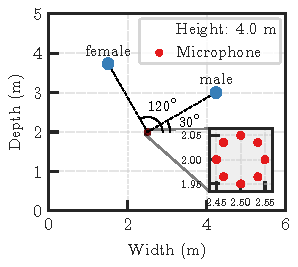
\includegraphics{figures/room_layout.pdf}
  \caption{Room layout.}%
  \label{fig:layout}
\end{figure}
\begin{itemize}
  \item 音源・マイク配置 (\cref{fig:layout}), 5音源5マイク
    % \begin{itemize}
    %   \item 前は2音源5マイクでやっていたが評価がよくわからなくなった…
    %     \begin{itemize}
    %       \item 参考:\href{https://github.com/onolab-tmu/overiva/blob/1cb3189112889ebfe2ccbbde0f55b1db6020fc48/overiva_sim.py#L200}{OverIVAの評価}\\
    %         分離信号の余ったチャネルをrandnで埋める
    %     \end{itemize}
    %   \item 分離音が複数チャネルに分かれる場合の評価方法?
    %   \item 分離されているとも言えるが,望ましい結果とは言えない…
    %   \item[$\Rightarrow$] 簡単のためにいったん決定条件でやり直した
    % \end{itemize}
  \item 残響時間: 約\SI{100}{\milli\second}
  \item マイク間隔: \SI{2}{\centi\metre}
  \item マイク回転角度: \SI{40}{\degree} at \SI{30}{\second}
  \item STFT: FFT長 4096, 1/2-shift, Hamming窓
  \item Projection back: \cref{alg:pb}, 参照マイク=1
  \item SI-SDRの参照信号: 各音源の音像(途中でマイクが回転する)
\end{itemize}

\subsection{結果}
% - 忘却係数 0.99 -> 回転にあまり追従しないようにしておく
\begin{itemize}
  \item 比較手法
    \begin{itemize}
      \item \Cref{alg:naive}: 通常のOnline AuxIVA (\textbf{Naive})
      \item \Cref{alg:reset}: 回転後に$\Demix _{\ft}, \cov _{\src,\ft}$を初期化 (\textbf{Reset})
      \item \Cref{alg:sfi}: 回転後に観測信号の回転を補償 (\textbf{RT-obs})\\
        $\Obs _{\ft} = \rotMat ^{\hermite} (\rotSpat _{\tframe}) \rot{\Obs} _{\ft}$
      \item \Cref{alg:coord}: 回転後に$\Demix _{\ft}, \cov _{\src,\ft}$を``座標変換'' (\textbf{RT-cov})\\
        $\rot{\Demix} _{\ft} \gets \Demix _{\ft} \rotMat ^{\hermite} (\rotSpat _{\tframe})$,\; $\rot{\cov} _{\src,\ft} \gets \rotMat (\rotSpat _{\tframe}) \cov _{\src,\ft} \rotMat ^{\hermite} (\rotSpat _{\tframe})$
    % \begin{itemize}
    %   \item $\cov _{\src,\ft[-1]}$はそれ以前のすべての観測の情報を含んでいるので,それだけに$\rotMat (\rotSpat)$をかけて,あとは観測をそのまま使って更新すればいいはず
    % \end{itemize}
    \end{itemize}
  \item パラメータ
    \begin{itemize}
      \item 初期値: $\Demix _{\freq,0} = \Eye\; (\forall \freq)$, $\cov _{\src,\freq,0} = 10^{-3}\times\Eye\; (\forall \src, \freq)$
      \item 忘却係数$\forget$: 0.9, 0.95, 0.98, 0.99
        \begin{itemize}
          \item 有効データ長 $\frac{1}{1 - \forget} = 10, 20, 50, 100$ となるよう選んだ
        \end{itemize}
      \item 音源モデル: 時変Gauss
      \item フレームごとの反復回数$\Itr$: 5
      \item 正則化: $\cov _{\src,\ft} \gets \cov _{\src,\ft} + 10 ^{-3} \Eye$
    \end{itemize}
\end{itemize}

\begin{figure}[t]
  \begin{minipage}[t]{\linewidth}
    \centering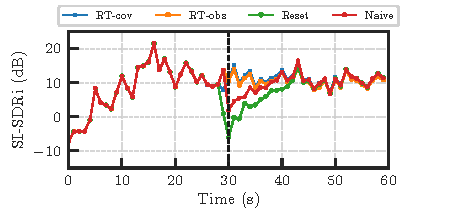
\includegraphics{figures/plots/online/Gauss_8000_fft4096_900.pdf}\subcaption{$\forget = 0.90 $}\label{fig:plot:gauss:900}
    \centering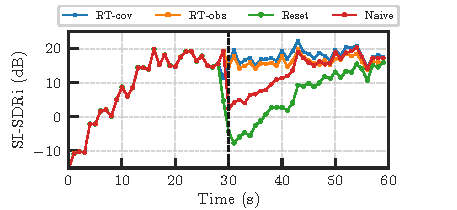
\includegraphics{figures/plots/online/Gauss_8000_fft4096_950.pdf}\subcaption{$\forget = 0.95 $}\label{fig:plot:gauss:950}
    \centering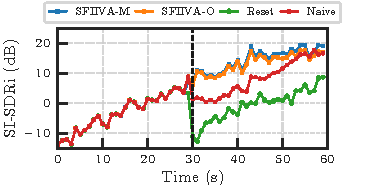
\includegraphics{figures/plots/online/Gauss_8000_fft4096_980.pdf}\subcaption{$\forget = 0.98 $}\label{fig:plot:gauss:980}
    \centering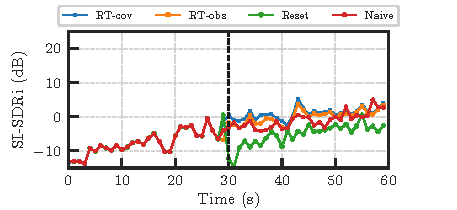
\includegraphics{figures/plots/online/Gauss_8000_fft4096_990.pdf}\subcaption{$\forget = 0.99 $}\label{fig:plot:gauss:990}
    % \centering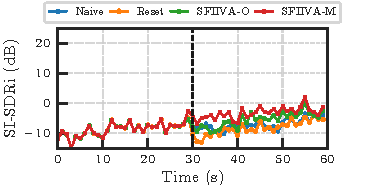
\includegraphics{figures/plots/online/Gauss_8000_fft4096_995.pdf}\subcaption{$\forget = 0.995$}\label{fig:plot:gauss:995}
  \end{minipage}
  \caption{Segmental SI-SDR improvements (SI-SDRi) every \SI{1}{\second} with $\Src = \Mic = 5$ and $\text{RT}_{60} \approx \SI{100}{\milli\second}$.}
\end{figure}

\paragraph{雑感・メモ}
\begin{itemize}
  \item 実験結果
    \begin{itemize}
      \item RT-cov
        \begin{itemize}
          \item マイク回転後も分離性能の低下がほとんどない
        \end{itemize}
      \item RT-obs
        \begin{itemize}
          \item RT-covとほとんど同じ
          \item 最終的な分離性能はRT-covにわずかに劣る
            \begin{itemize}
              \item 音源分離はマイク回転を補償した観測信号,\\性能評価はマイク回転ありの音像を用いているため?
            \end{itemize}
        \end{itemize}
      \item Reset
        \begin{itemize}
          \item 回転後に大きく性能が低下
          \item 回転後は徐々に収束
          \item 忘却係数$\forget$が1に近づくほど回転前後の性能差が大きくなる
        \end{itemize}
      \item Naive
        \begin{itemize}
          \item 回転後に大きく性能が低下,低下の幅はResetよりも小さく,ほとんどすべての忘却係数について同じくらい
        \end{itemize}
    \end{itemize}
  \item その他
    \begin{itemize}
      \item FFT長2048以下,忘却係数0.95以下で$\cov _{\src,\ft} ^{-1}$が発散する
    \end{itemize}
\end{itemize}

\paragraph*{疑問}
\begin{itemize}
  \item オンラインAuxIVAでの共分散行列 ``座標変換'' ?\\ バッチの場合と勝手が違う気がする…\\
    マイクは $\tframe \leq \rotFra - 1$ で基準位置,
    $\tframe \geq \rotFra$ で回転後とする.
    \begin{align*}
      \rot{\cov} _{\src,\ft} &= \forget \cov _{\src,\ft[-1]} + (1 - \forget) \weight(\var _{\src,\tframe}) \rot{\Obs} _{\ft} \rot{\Obs} _{\ft} ^{\hermite} \\
                             &= \forget ^{\tframe} \cov _{\src,\freq,0}
                                + \sum _{i = 1} ^{\rotFra - 1} \forget ^{\tframe - i} (1 - \forget) \weight(\var _{\src,i}) \Obs _{\freq,i} \Obs _{\freq,i} ^{\hermite} \\
                             &\qquad + \sum _{j = \rotFra} ^{\tframe} \forget ^{\tframe - j} (1 - \forget) \weight(\var _{\src,j}) \rot{\Obs} _{\freq,j} \rot{\Obs} _{\freq,j} ^{\hermite}
    \end{align*}
  \item 音場補間,座標変換のいい感じの名前?ロボット工学の用語でワールド座標系,ロボット座標系などがあるが,これをもじって簡潔に言い表せないか?
\end{itemize}

\paragraph*{TODO}
\begin{itemize}
  \item 忘却係数を周波数ごとに設計
    \begin{itemize}
      \item 音場補間は高周波数帯では動かないので高い周波数は早く忘れるようにする?
    \end{itemize}
  \item 周波数ごとのSDRの計算
  \item 音場補間あり・なしでそれぞれ計算した分離行列との差分を可視化
  \item 実際のマイク回転角度と推定した回転角度に誤差をつけた場合の実験
\end{itemize}

\begin{algorithm}{Online AuxIVA (OIVA)}{naive}
  \textbf{Input:} $\{\Obs _{\ft}\} _{\freq},\, \{\Demix _{\ft[-1]}\}_{\freq},\, \{\cov _{\src,\ft[-1]}\}_{\src,\freq}$\\
  % \textbf{Output:} $\Est _{\ft},\, \Demix _{\ft},\, \cov _{\src,\ft}\; (\forall \src,\freq)$
  \textbf{Output:} $\{\Demix _{\ft}\}_{\freq},\, \{\cov _{\src,\ft}\}_{\src,\freq}$
  \begin{pseudo}
    {$\Demix _{\ft}$} $\gets$ $\Demix _{\ft[-1]}$ \ct{$(\forall \freq)$} \\
    for $\itr = 1,\, \dots,\, \Itr$ \\+
      for $\src = 1,\, \dots,\, \Src$ \\+
        {$\var _{\src,\tframe}$} $\gets$ $\sqrt{\sum _{\freq} \abs{\demix _{\src,\ft} ^{\hermite} \Obs _{\ft}} ^2}$ \\
        {$\cov _{\src,\ft}    $} $\gets$ $\forget \cov _{\src,\ft[-1]} + (1 - \forget) \weight(\var _{\src,\tframe}) \Obs _{\ft} \Obs _{\ft} ^{\hermite}$ \ct{$(\forall \freq)$}\\-
      forall $\src = 1, \dots, \Src$ \\+
        {$\demix _{\src,\ft}$} $\gets$ $\left(\Demix _{\ft} \cov _{\src,\ft}\right) ^{-1} \eye _{\src}$ \ct{$(\forall \freq)$}\\
        {$\demix _{\src,\ft}$} $\gets$ $\dfrac{\demix _{\src,\ft}}{\sqrt{\demix _{\src,\ft} ^{\hermite} \cov _{\src,\ft} \demix _{\src,\ft}}}$ \ct{$(\forall \freq)$}
        % {$\Est _{\ft}  $} $\gets$ $\Demix _{\ft} \Obs _{\ft}$ \ct{$(\forall \freq)$}
  \end{pseudo}
\end{algorithm}
\begin{algorithm}{Online AuxIVA with reset (\textbf{Reset})}{reset}
  \begin{pseudo}
    for $\tframe = 1,\, \dots,\, \rotFra - 1$ \\+
      $\{\Demix _{\ft}\}_{\freq},\, \{\cov _{\src,\ft}\} _{\src,\freq} \gets$ \pr{OIVA}(\{\Obs _{\ft}\} _{\freq}, \{\Demix _{\ft[-1]}\}_{\freq},\, \{\cov _{\src,\ft[-1]}\} _{\src,\freq}) \\-
    {$\Demix _{\freq,\rotFra - 1}$} $\gets$ $\Eye$ \ct{$(\forall \freq)$} \\
    {$\cov _{\src,\freq,\rotFra - 1}$} $\gets$ $\varepsilon \Eye$ \ct{$(\forall \src,\freq)$} \\
    for $\tframe = \rotFra,\, \dots,\, \Tframe$ \\+
      $\{\Demix _{\ft}\}_{\freq},\, \{\cov _{\src,\ft}\} _{\src,\freq} \gets$ \pr{OIVA}(\{\Obs _{\ft}\} _{\freq}, \{\Demix _{\ft[-1]}\}_{\freq},\, \{\cov _{\src,\ft[-1]}\} _{\src,\freq})
  \end{pseudo}
\end{algorithm}

\begin{algorithm}{Online AuxIVA with sound field interpolation for observed signal (RT-obs)}{sfi}
  \begin{pseudo}
    for $\tframe = 1,\, \dots,\, \rotFra - 1$ \\+
      $\{\Demix _{\ft}\}_{\freq},\, \{\cov _{\src,\ft}\} _{\src,\freq} \gets$ \pr{OIVA}(\{\Obs _{\ft}\} _{\freq}, \{\Demix _{\ft[-1]}\}_{\freq},\, \{\cov _{\src,\ft[-1]}\} _{\src,\freq}) \\-
    $\rotMat (\rotSpat _{\tframe})$ $\gets$ \pr{CalcRotationMatrix}(\Mic, \rotSpat _{\tframe}) \\
    for $\tframe = \rotFra,\, \dots,\, \Tframe$ \\+
      $\refpos{\Obs} _{\ft} \gets \rotMat ^{\hermite} (\rotSpat _{\tframe}) \Obs _{\ft}$ \ct{$(\forall \freq)$} \\
      $\{\Demix _{\ft}\}_{\freq},\, \{\cov _{\src,\ft}\} _{\src,\freq} \gets$ \pr{OIVA}(\{\refpos{\Obs} _{\ft}\} _{\freq}, \{\Demix _{\ft[-1]}\}_{\freq},\, \{\cov _{\src,\ft[-1]}\} _{\src,\freq})
  \end{pseudo}
\end{algorithm}
\begin{algorithm}{Online AuxIVA with ``transformation''}{coord}
  \begin{pseudo}
    for $\tframe = 1,\, \dots,\, \rotFra - 1$ \\+
      $\{\Demix _{\ft}\}_{\freq},\, \{\cov _{\src,\ft}\} _{\src,\freq} \gets$ \pr{OIVA}(\{\Obs _{\ft}\} _{\freq}, \{\Demix _{\ft[-1]}\}_{\freq},\, \{\cov _{\src,\ft[-1]}\} _{\src,\freq}) \\-
    $\rotMat (\rotSpat _{\tframe})$ $\gets$ \pr{CalcRotationMatrix}(\Mic, \rotSpat _{\tframe}) \\
    {$\rot{\Demix} _{\freq,\rotFra - 1}$} $\gets$ $\Demix _{\freq,\rotFra - 1} \rotMat ^{\hermite} (\rotSpat)$ \ct{$(\forall \freq)$} \\
    {$\rot{\cov} _{\src,\freq,\rotFra - 1}$} $\gets$ $\rotMat (\rotSpat _{\tframe}) \cov _{\src,\freq,\rotFra - 1} \rotMat ^{\hermite} (\rotSpat _{\tframe})$ \ct{$(\forall \src,\freq)$} \\
    for $\tframe = \rotFra,\, \dots,\, \Tframe$ \\+
      $\{\rot{\Demix} _{\ft}\}_{\freq},\, \{\rot{\cov} _{\src,\ft}\} _{\src,\freq} \gets$ \pr{OIVA}(\{\Obs _{\ft}\} _{\freq}, \{\rot{\Demix} _{\ft[-1]}\}_{\freq},\, \{\rot{\cov} _{\src,\ft[-1]}\} _{\src,\freq})
  \end{pseudo}
\end{algorithm}

\begin{algorithm}{Projection back (online)}{pb}
  \textbf{Input:} $\Obs _{\ft}$, $\Demix _{\ft}$, reference microphone index $\ell$\\
  \textbf{Output:} Scale-restored output signal $\Est _{\ft}$
  \begin{pseudo}
    for $\tframe = 1,\, \dots,\, \Tframe$ \\+
      for $\freq = 1,\, \dots,\, \Freq$ \\+
        $\begin{bmatrix} \steer _{1,\ft} & \dots & \steer _{\Mic,\ft} \end{bmatrix} \eqqcolon \Steer _{\ft} \gets \Demix _{\ft} ^{-1}$ \\
        % $\tilde{\Demix} _{\ft} \gets \mathrm{diag}(\steer _{\ell,\ft}) \Demix _{\ft}$ \\
        % \nf{$\phantom{\tilde{\Demix} _{\ft} \gets} = \begin{bmatrix} a _{1,\ell,\ft} & \dots & 0 \\ \vdots & \ddots & \vdots \\ 0 & \dots & a _{\Src,\ell,\ft} \end{bmatrix} \Demix _{\ft}$} \\
        $\Est _{\ft} \gets \mathrm{diag}(\steer _{\ell,\ft}) \Demix _{\ft} \Obs _{\ft}$
  \end{pseudo}
\end{algorithm}

\section{Conclusion}\label{sec:conclusion}
% 本研究では,円状等間隔マイクロホンアレイにおける音場補間をブラインド音源分離に応用した.
% シミュレーション実験により,音場補間が円状等間隔マイクロホンアレイの回転に対するOIVAの頑健性を改善させたことを確認した.
% 今後は本手法の自己回転角度推定 \cite{Lian:2021:APSIPA} との組み合わせや,実時間処理への拡張などに取り組む.
In this study, sound field interpolation for an equally spaced circular microphone array (CMA) was applied to online auxiliary-function-based independent vector analysis (OIVA).
Simulation experiments have confirmed that sound field interpolation improved robustness of OIVA against the rotation of CMA.
Future work includes combining this method with self-rotation angle estimation \cite{Lian:2021:APSIPA} and extending it to real-time processing.

\section*{Biographies}

\noindent\normalsize\textbf{Taishi Nakashima}
received his B.E. in Engineering from Osaka University, Osaka, Japan, in 2019 and his M.S. in Informatics from Tokyo Metropolitan University, Tokyo, Japan, in 2021.
He is pursuing a Ph.D. at Tokyo Metropolitan University and is also a recipient of the JSPS Research Fellowship (DC1) from April 2021.
He is an esteemed Student Member of the Acoustical Society of Japan (ASJ) and the IEEE Signal Processing Society (SPS).
He received the 24th Best Student Presentation Award of ASJ and the 16th IEEE SPS Japan Student Conference Paper Award in 2022, and Top 3\% Recognition at ICASSP 2023.
His research interests primarily focus on blind source separation and acoustic signal processing.
\\

\noindent\normalsize\textbf{Yukoh Wakabayashi}
received the B.E. and M.E. degrees from Osaka University, Osaka, Japan, in 2008 and 2010, respectively, and Ph.D. degree from Ritsumeikan University, Shiga, Japan, in 2017.
He joined Rohm, Inc., Kyoto, Japan, in 2010, and was an assistant researcher with Kyoto University from 2012 to 2014.
He was a recipient of the JSPS Research Fellowship for Young Scientists DC2 from 2016 to 2017.
He was an affiliate assistant professor with Ritsumeikan University from 2018 to 2020.
He is currently an assistant professor with the Department of Computer Science and Engineering, Toyohashi University of Technology, Aichi, Japan, and the Faculty of Systems Design, Tokyo Metropolitan University, Tokyo, Japan.
His research interests include acoustic signal processing, speech phase processing, array signal processing, and speaker diarization.
He is a member of the Institute of Electrical and Electronics Engineers, the Institute of Electronics, Information and Communication Engineers, and Acoustical Society of Japan.
\\

\noindent\normalsize\textbf{Nobutaka Ono}
received his B.E., M.S., and Ph.D. degrees from the University of Tokyo, Japan, in 1996, 1998, and 2001, respectively.
He became a research associate in 2001 and a lecturer in 2005 at the University of Tokyo.
He moved to the National Institute of Informatics in 2011 as an associate professor and then to Tokyo Metropolitan University in 2017 as a full professor.
His research interests include acoustic signal processing, especially microphone array processing, source localization and separation, machine learning, and optimization algorithms.
He is a member of IEEE, EURASIP, APSIPA, IPSJ, IEICE, and ASJ.
He was a member of IEEE Audio and Acoustic Signal Processing (AASP) Technical Committee from 2014 to 2019.
He served as Associate Editor of IEEE Transactions on Audio, Speech, and Language Processing from 2012 to 2015.
He received the best paper award at APSIPA ASC in 2018 and 2021 and Sadaoki Furui Prize Paper Award from APSIPA in 2021.

\printbibliography

\end{document}
